\section{Solving quadratic equations -- Practice exercises}

\bigskip

Formula referenced in the worksheets:

\bigskip
 \framebox{
 \begin{minipage}[c]{.85\textwidth}  
~ \bigskip \\  \textsc{Quadratic Formula:} \quad The equation $aT^2+bT+c=0$ has solutions \\ $$T = \frac{-b}{2a} \pm \frac{\sqrt{b^2-4ac}}{2a}$$ \bigskip
\end{minipage}
}
\bigskip

\begin{enumerate}

\item A high-jumper jumps so that the height, $H$ feet, of the point on his back that must clear the bar after $T$ seconds is given by the equation
$$H = 3.5 + 16T -16T^2$$
\begin{center}
\scalebox {.8} {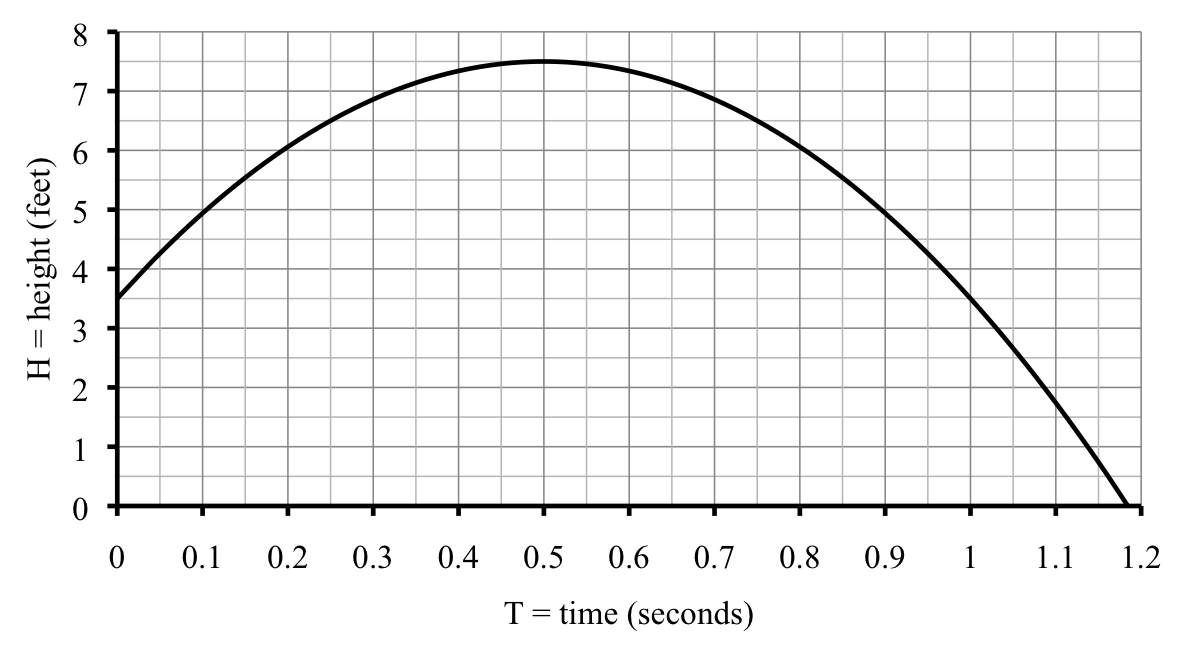
\includegraphics [width = 6in] {highjumper.png}}
\end{center}

\begin{enumerate}
\item When would the high-jumper hit the ground (if there were no pit)?  Ouch!   Use the \textsc{Quadratic Formula} to find the answer.  Use the graph to check. \vfill

\newpage %%%%%%
~\hspace{-.5in} \emph{The problem continues \ldots}

\item The high jump pit is 2 feet off the ground.  When does the high-jumper land in the pit?  Use the \textsc{Quadratic Formula} to find the answer and the graph to check. \vfill
\item How high a bar can the high-jumper clear?  Find the maximum height of that point above ground by evaluating at $\displaystyle T=\frac{-b}{2a}$.  Use the graph to check.  \vfill
\end{enumerate}

\newpage %%%%%%

\item The art museum opened in 1920.  After an initial rush to see the great holdings, attendance dropped for awhile.  But then attendance began to rise again and has risen since.  The number of annual visits $N$ is approximated by the equation $$N= 51Y^2-840Y+\text{3,700}$$ 
where $Y$ is the year since 1920.

\begin{enumerate}
\item Calculate the missing values in the table.
\begin{center}
\begin{tabular} {|c ||c |c |c |c |c |c |c |} \hline
year & 1920 & 1925 & 1930 & 1935 & 1940 & 1945 & 1950 \\ \hline
$Y$  &0 & 5& 10 & 15 & 20 & 25 & 30  \\ \hline
$V$ & \text{3,700} & \hspace{.5in}~ & 400 & \text{2,575} & \text{7,300} & \hspace{.5in}~  & \text{24,400}\\
&&&&&&&  \\ \hline
\end{tabular}
\end{center}
\item Draw a graph of the function.
\begin{center}
\scalebox {.8} {
\includegraphics [width = 6in] {GraphPaper.jpg}}
\end{center}
\bigskip
\item In what year did the number of visitors first pass \text{30,000} in a year?  Estimate the value from your graph.  Then set up and solve a quadratic equation. \vfill

\newpage %%%%%%
~\hspace{-.5in} \emph{The problem continues \ldots}

\item According to this equation, in what year was the number of annual visits the smallest?  For that year, what were the number of visits?   Use $\displaystyle T=\frac{-b}{2a}$\vfill
\item Explain why $N$ never equals 0.  \vfill
\item So, what actually happens when you try to use the \textsc{Quadratic Formula} to solve for $N=0$?\vfill

\end{enumerate}

\newpage %%%%%%

\item The profit \$$P$ from selling $M$ tanks of milk is described by the equation $$P=-2M^2+\text{2,000}M-\text{80,000}$$
\begin{enumerate}
\item The graph is drawn below.  Explain why negative numbers make sense. \vfill
\begin{center}
\scalebox {.9} {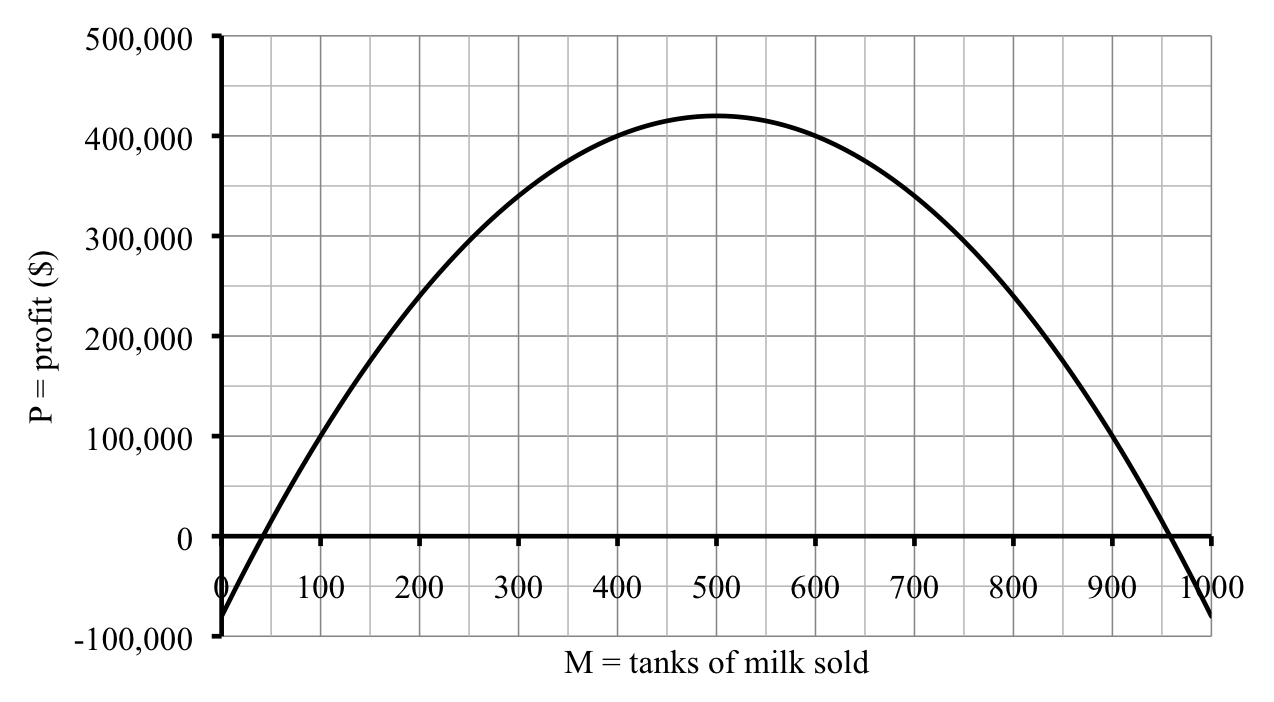
\includegraphics [width = 6in] {milk.png}}
\end{center}
\item How much milk must be sold for the company to \textbf{break even}, meaning having \$0 profit? Guess from the graph and check using the equation. \vfill
\item For practice, set up and solve a quadratic equation to find the break even point.  \vfill \vfill \vfill

\newpage %%%%%%
~\hspace{-.5in} \emph{The problem continues \ldots}

\item How many tanks of milk would they need to sell to keep profits over \$\text{400,000}?  Set up and solve a quadratic equation to find the answer.  Then check that it agrees with your graph.   Your answer should be in the form of an inequality. \vfill
\end{enumerate}

\newpage %%%%%%

 \item Urban community gardens are catching on.  What was once an abandoned lot down the block is now a thriving 10'$\times$25' vegetable and berry garden for the neighborhood. One neighbor  volunteered to donate  gravel to make a path around the garden.  The path will be 3 inches deep and the same width all around.   
\begin{center}
\scalebox {.4} {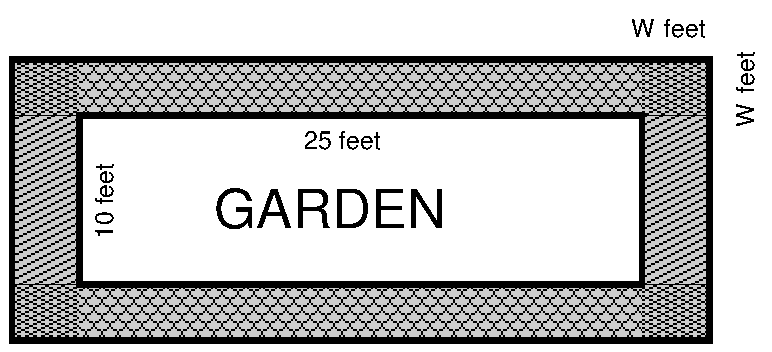
\includegraphics{GravelPath.pdf}}
\end{center}
The amount of gravel we need ($G$ cubic feet) is given by the equation  $$G = W^2 + 17.5W$$
where $W$ is the width of the path in feet.  For example, a path 4 feet wide requires 86 cubic feet of gravel, as you can check.
\hfill \emph{Story also appears in 2.3 and 2.4 Exercises}
\begin{enumerate}
\item  If the neighbor donates 60 cubic feet of gravel, how wide a path can they build?  Set up and solve a quadratic equation to find the answer to two decimal places in feet. Then convert your answer into inches. \vfill
\item Gravel is measured by the \textbf{yard}, which is short for cubic yard.  There are 27 cubic feet in 1 cubic yard.  If the neighbor donates three yards of gravel, how wide a path can they build? Set up and solve a quadratic equation to find the answer to two decimal places in feet. Then convert your answer into inches. \vfill
\item What would it mean to solve the equation to find where $G=0$?  Can you tell what the answer is from the equation (without actually solving)? \bigskip
\end{enumerate}

\end{enumerate}

